\section{Inbetriebnahme}
Hier werden die Inbetriebnahmetests beschrieben.

\subsection{Tests Einzelkomponenten}
Kurz nach der Endmontage werden die einzelnen Komponenten getestet. Eine erste 
Inbetriebnahme des Ballnachschubs zeigt, dass die Funktion gewährleistet ist. 
Das Drehmoment des Servomotors genügt um die 5 Bälle nach oben zu befördern. 
Die Geschwindigkeit des Ballnachschubs kann mit der Betriebsspannung des 
Motors eingestellt werden, allerdings ist sie auf ca. 12V begrenzt, da 
anderenfalls der Motor überlastet wird.

\noindent
Der BLDC Motor kann bereits angesteuert werden. Dabei wird die Drehzahl über 
ein Netzgerät eingestellt. Hier zeigt sich, dass der Pneu eine Unwucht hat. Leider 
kann diese Unwucht nicht mit konventionellen Massnahmen behoben werden, das es 
sich um Ungenauigkeiten in der Dicke und in der Form handelt. Mit der 
erforderten Drehzahl für die Schussweite von ca. 2m wirkt sich die Unwucht 
jedoch nicht auf die Konstruktion aus.

\noindent
Mit dieser Konfiguration werden die ersten Ballwürfe gemacht. Zuerst wird der 
Ballnachschub sehr langsam eingestellt, so dass die Drehzahl des BLDC-Motors 
nach einem Schuss wieder auf die Anfangsdrehzahl gestiegen ist. Da die 
Streuung der Reichweite ungewöhnlich stark variiert (ca. 0.5m), haben wir auf 
der Gegenseite des Rades ein Stück Gummi aufgeklebt, so dass die Reibung des 
Tennisballs grösser ist. So wird die Streuung auf ca. $\pm$0.1m verkleinert. 

\begin{figure}[h!]          
	\centering             
	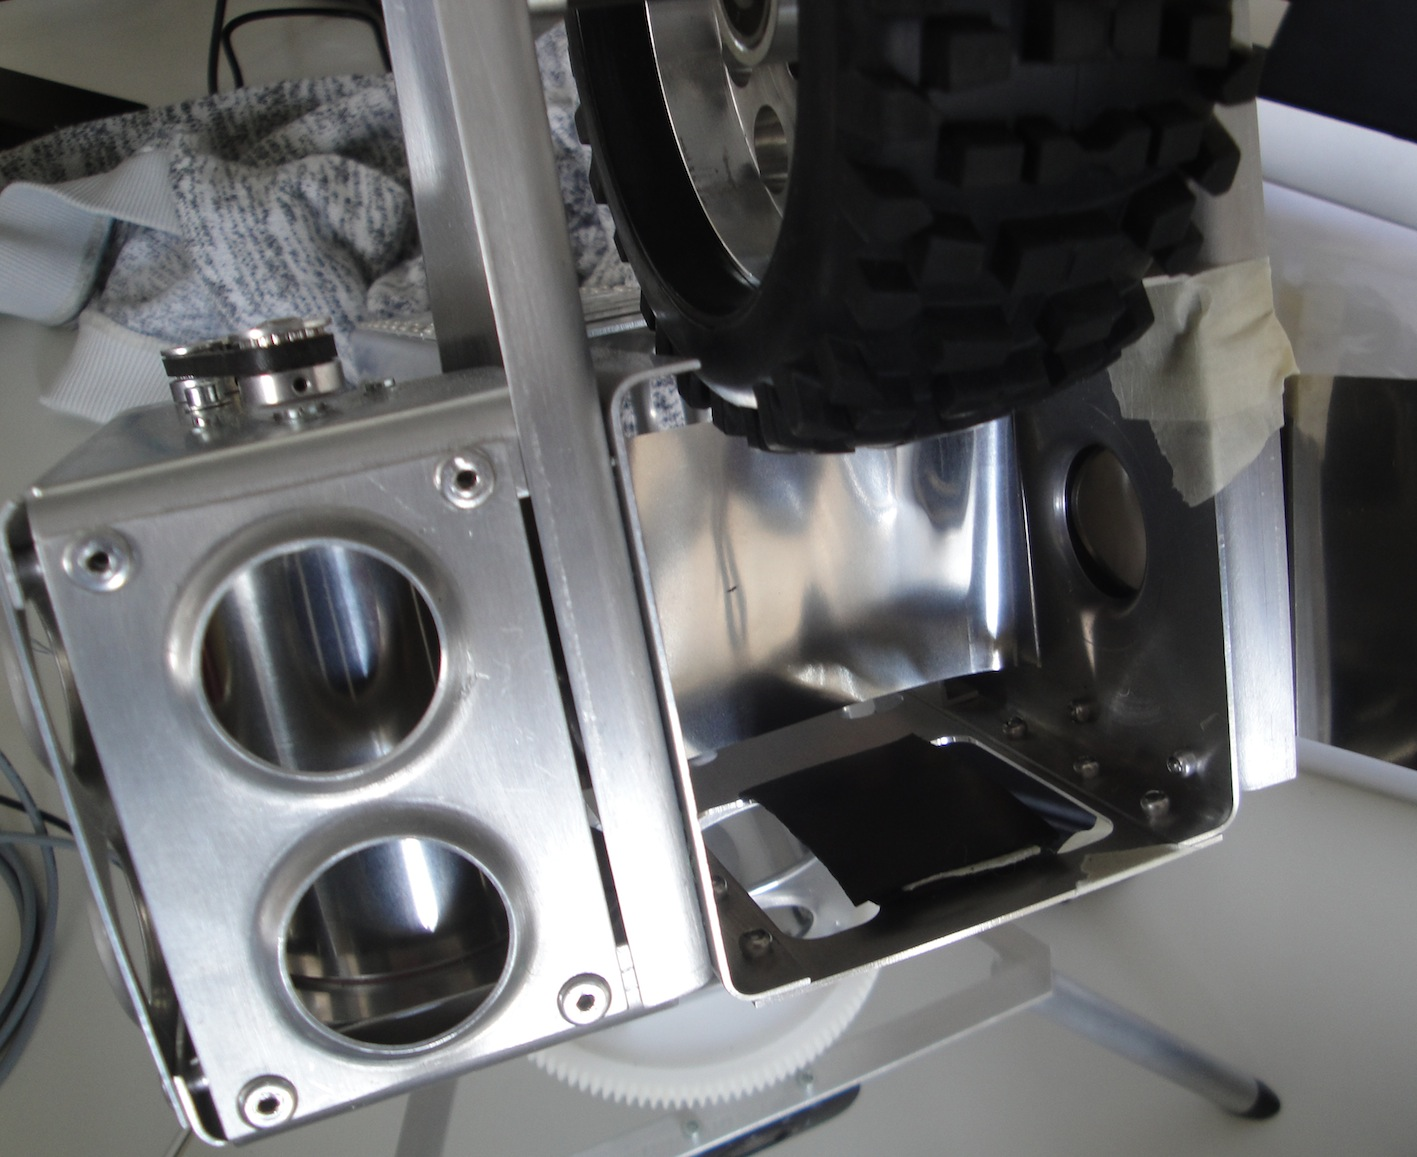
\includegraphics[width=0.5\textwidth]{fig/Bild_Gummi.JPG}
	\caption{Gummi zur Erhöhung der Reibung}
	\label{fig:Gummi}        
\end{figure}

\noindent
In weiteren Tests werden die Bälle möglichst schnell nacheinander geschossen, 
so dass sich die Drehzahl des BLDC Motors nicht mehr ganz erholen kann. 
Komischerweise wird so die Streuung noch kleiner (nicht mehr von Auge 
abschätzbar). Drei weitere Tests mit Wettbewerbsbedingungen (Distanz und Höhe 
des Korbes) und mit schnellem Ballnachschub zeigen, dass die Genauigkeit sehr 
hoch ist, alle Bälle landen im Korb. Gegebenenfalls könnte mit einem anderen 
Pneu die Genauigkeit noch erhöht werden.

\noindent
Die Drehvorrichtung funktioniert und ist sehr schnell. Bei ersten Tests (ohne 
Tennisbälle) konnte innerhalb einer Sekunde mehr als eine Umdrehung gemacht 
werden. Schlussendlich muss sich der Turm nur um ca. 16$^\circ$ drehen, somit 
sollte ca. 1/5 Sekunde reichen um die Richtung einzustellen.

\clearpage
\subsection{Tests Gesamtsystem}
\subsubsection{Ablauf}
Die Tests des Gesamtsystems werden durchgeführt, um das Zusammenspiel und 
richtige Funktionieren der einzelnen Komponenten zu gewährleisten. Dazu wird 
eine Bluetooth-Verbindung mit dem Gerät hergestellt. Da der BLDC-Motor beim 
Wettkampf bereits gestartet sein darf, wird dieser mittels Eingabefeld der 
Applikation bereits vor dem Wettkampfstart auf eine Drehzahl von 
1400\si{\per\minute} konfiguriert.

\noindent
Anschliessend wird mittels Bilderkennung ein aktuelles Foto des Spielfelds 
geschossen. Auf diesem Foto wird per Mausziehen der Bereich des Spielfeldes 
ausgewählt. Wird nun das Startsignal gegeben, kann ein Button gedrückt werden, 
der dann die Ausrichtung des Geräts übernimmt und den Ballnachschub nach einer 
Verzögerung von $\frac{\text{Anzahl Schritte}}{20}$ in Bewegung setzt.

\noindent
Sind alle Bälle geworfen, wird ein String an alle Observer des 
\verb?BluetoothReceivers? gesendet. Enthält dieser String "fin", so heisst 
dies, dass das Gerät alle Bälle verschossen hat und somit das Endsignal 
ausgelöst werden kann. Nach dem Endsignal ist der Test beendet.

\subsubsection{Resultate}
\noindent
Die ersten Tests zeigen, dass die Ballnachführung nicht zeitgleich mit 
dem Ausrichten in Bewegung gesetzt werden darf, da ansonsten der erste Ball 
nicht trifft, wenn der Korb am Rand des Spielfelds steht. Integrationstests 
dieser beiden Komponenten zeigen, dass die optimale Verzögerungszeit für den 
Start der Ballnachführung nach dem Ausrichten bei $\frac{\text{Anzahl 
Schritte}}{20}$ liegt. 

\noindent
Weitere Tests zeigen, dass bei der anfangs konfigurierten Drehzahl von 
1372\si{\per\minute} der erste Ball bei einem Ausrichtungswinkel von mehr als 
$16^\circ$ nicht trifft. Dies liegt daran, dass der erste Ball mit einer 
niedrigeren Geschwindigkeit an das Rad geführt wird, als die anderen Bälle. 
Dieses Problem ist nun behoben worden, indem der BLDC-Motor anfangs auf 
1400\si{\per\minute} eingestellt wird und zeitgleich zum Ausrichten auf 
1372\si{\per\minute} heruntergefahren wird. Bei Tests mit dieser Konfiguration 
treffen alle Bälle den Korb.
